\documentclass[11pt]{article}

% --- Packages (kept deliberately simple for portability) ---
\usepackage[margin=1in]{geometry}
\usepackage{amsmath,amssymb,amsthm}
\usepackage{graphicx}
\usepackage{booktabs}
\usepackage{array}
\usepackage{caption}
\usepackage{xcolor}
\usepackage{enumitem}
\usepackage[hidelinks]{hyperref}

\captionsetup{font=small,labelfont=bf}

\newtheorem{theorem}{Theorem}
\newtheorem{corollary}{Corollary}
\newtheorem{assumption}{Assumption}

\newcommand{\argmax}{\operatorname*{arg\,max}}
\newcommand{\note}[1]{\textcolor{gray}{#1}}

\title{\textbf{Beyond Confidence: Counterfactual Stability as a Second Axis
of Neural Network Reliability}\\[0.4em]
\large Finite-Candidate Shortcut Audit and Repair in Pretrained
Vision--Language Models}

\author{Rohan Nagaram}
\date{\today}

\begin{document}
\maketitle

\begin{abstract}
\noindent
Confidence is the default signal practitioners use to decide whether to trust a
neural network's prediction. But confidence alone cannot distinguish genuine
uncertainty from \emph{shortcut dependence}: a model can be confidently right for
the wrong reason, relying on a spurious feature that happens to correlate with the
label. We study \emph{Counterfactual Instability Certificates} (CIC), a per-example
signal that measures how much a prediction changes under \emph{label-preserving}
interventions on a finite candidate set of hypothesized shortcuts. CIC is not a
replacement for confidence; it is a second, orthogonal axis of reliability.

Our main empirical results are on real pretrained OpenCLIP (\texttt{ViT-B-32},
\texttt{laion2b\_s34b\_b79k}; no fake backend used for any headline evidence).
On a held-out hard multi-decoy text-overlay benchmark, misleading text reduces
accuracy from near-perfect clean/aligned performance to $25.0\%$. Non-oracle CIC
region scoring repairs accuracy to $75.0\%$, versus $33.1\%$ for a matched random
text-region control, while keeping the clean-safe accuracy drop to $1.0\%$. A
\emph{full benchmark-resampling audit} over three independently regenerated
benchmark instances (with distinct image and metadata hashes) reproduces the
effect: CIC's advantage over the matched random control ranges $0.39$--$0.54$
(mean $0.46$) with a mean clean drop of $\approx 0.01$. In a
\emph{failure-conditioned} evaluation on $50$ verified shortcut failures (where
original accuracy is $0$ by construction), CIC repairs $96$--$98\%$ of cases
versus $\approx 11.2\%$ for matched random text repair.

On theory, the \emph{global} input-independent embedding-additivity assumption is
\textbf{not} supported for OpenCLIP text overlays --- the per-image shortcut shift
clusters more tightly by object class than by shortcut value. The weaker
\emph{residual-to-clean}, per-input class-balance premise is supported most clearly
for oracle neutralization and directionally for CIC-selected regions, making the
recovery theorem a plausible but conservative mechanism account for text-overlay
repair. We retain a clear negative boundary: the frozen
text-selected policy did \textbf{not} transfer to a non-text colored-symbol
watermark shortcut. The scope is strictly finite-candidate interventions: this work
makes no claim of open-world shortcut discovery, exact bounding-box localization,
general robustness, or cross-shortcut generalization.
\end{abstract}

\tableofcontents

% =====================================================================
\section{Introduction}
% =====================================================================
A deployed classifier that is wrong is a problem; a classifier that is
\emph{confidently} wrong, for a reason the operator cannot see, is a safety hazard.
Modern networks are routinely calibrated and gated on confidence, yet confidence
answers only one question: \emph{how sure is the model?} It is silent on a second,
equally important question: \emph{does that certainty depend on evidence that
actually determines the label, or on a shortcut?}

A \emph{shortcut} (or spurious feature) is predictive of the label in the training
distribution but is not causally necessary for the true class~\cite{geirhos2020shortcut}.
Vision--language models are a vivid example: pretrained CLIP can be flipped by a
small piece of overlaid text~\cite{goh2021multimodal,radford2021clip}, predicting the
written word rather than the depicted object --- often with high confidence. A
confidence-only monitor cannot catch this, because the failure is confident.

This report develops and evaluates a complementary signal. A
\textbf{Counterfactual Instability Certificate} (CIC) measures how much a
prediction moves when a hypothesized shortcut is changed while the label-defining
content is preserved. A reliable prediction should be \emph{stable} under such
label-preserving interventions; a shortcut-dependent prediction is \emph{unstable}.
We argue that confidence and counterfactual stability are two axes of a
\emph{reliability plane}, and that the most dangerous quadrant --- high confidence,
low stability --- is exactly the one confidence cannot police.

\paragraph{Contributions and honest scope.}
\begin{enumerate}[leftmargin=1.4em,itemsep=2pt]
\item A per-example, model-agnostic reliability signal (CIC) and a two-axis
reliability plane that separates uncertainty from shortcut dependence
(Sections~\ref{sec:cic}--\ref{sec:plane}).
\item A real-pretrained-OpenCLIP hard multi-decoy benchmark with a non-oracle
finite-candidate audit-and-repair workflow, plus a full benchmark-resampling audit,
a failure-conditioned evaluation, and a second controlled shortcut family (a
non-text semantic-decoy icon) on which the same method passes all gates at $n=64$
and $n=128$ as supporting evidence (Sections~\ref{sec:design}--\ref{sec:results}).
\item A conditional, finite-candidate recovery theory, gated on \emph{measured}
validation metrics: the strong global-additivity form fails for CLIP, but the
weaker per-input class-balance premise the theorem needs is supported
(Section~\ref{sec:theory}).
\item Retained negative results: no cross-shortcut transfer to watermarks; no exact
localization; no general robustness (Section~\ref{sec:negative}).
\end{enumerate}
The framework is a finite-candidate \emph{audit-and-repair} tool. It is
\textbf{not} open-world shortcut discovery, \textbf{not} exact localization, and
\textbf{not} a general robustness method.

\paragraph{Final claims at a glance.}
\begin{center}
\fbox{\begin{minipage}{0.95\linewidth}
\small
\textbf{Supported claims.}
\begin{enumerate}[leftmargin=1.6em,itemsep=1pt,topsep=2pt]
\item CIC is a second axis of reliability, complementary to confidence.
\item In finite-candidate text-region settings, non-oracle CIC repair substantially
outperforms matched random controls on real pretrained OpenCLIP
($0.250\to0.750$ vs.\ $0.331$ matched random).
\item The result survives a full benchmark-resampling audit (CIC$-$random gap
$0.39$--$0.54$, mean $0.46$; clean drop $\approx 0.01$).
\item On verified failure-conditioned examples (original accuracy $0$ by
construction), CIC repairs most failures ($0.96/0.98$), but the subset is selected
by failure.
\item The theory is supported through per-input class-balance, not global
additivity.
\item Cross-shortcut transfer to a colored-symbol watermark shortcut failed.
\end{enumerate}
\textbf{Unsupported (explicitly \emph{not} claimed).}
\begin{enumerate}[leftmargin=1.6em,itemsep=1pt,topsep=2pt]
\item Open-world shortcut discovery.
\item Exact bounding-box localization.
\item General robustness.
\item Cross-shortcut generalization.
\end{enumerate}
\end{minipage}}
\end{center}

% =====================================================================
\section{Background and Related Work}\label{sec:related}
% =====================================================================
This project does not claim to invent shortcut learning, spurious correlations, or
counterfactual invariance. Its contribution is an operational per-example
reliability certificate, a two-axis plane, baseline-tested shortcut-failure
regimes, and a finite-candidate audit/repair workflow.

\paragraph{Shortcut learning and spurious correlations.}
Shortcut learning is a well-documented failure mode: models exploit background,
texture, source, or annotation artifacts that correlate with labels in one
environment and fail under shift~\cite{geirhos2020shortcut}. Benchmarks such as
Colored MNIST, Waterbirds, and CelebA attribute shifts separate a stable label
feature from a correlated nuisance feature, and overparameterization can exacerbate
reliance on the spurious feature~\cite{sagawa2020investigation}.

\paragraph{Robust optimization.}
Group DRO~\cite{sagawa2020groupdro} and IRM~\cite{arjovsky2019irm} target invariance
or worst-group robustness \emph{during training}, typically requiring group labels
or multiple environments. CIC is instead a \emph{diagnostic and audit} signal that
applies to a fixed, pretrained model when candidate interventions are available; it
does not require retraining.

\paragraph{Counterfactual invariance and augmented data.}
Counterfactually-augmented data~\cite{kaushik2020counterfactual} and counterfactual
invariance~\cite{veitch2021counterfactual} ask whether predictions should remain
stable under label-preserving edits. CIC uses that idea at \emph{evaluation time} as
a per-example certificate rather than as a training objective.

\paragraph{CLIP typographic attacks.}
CLIP and related VLMs are vulnerable to typographic / text-overlay
cues~\cite{radford2021clip,goh2021multimodal}. We use this phenomenon as a
controlled, finite-candidate shortcut benchmark on real pretrained
OpenCLIP~\cite{ilharco2021openclip,schuhmann2022laion5b}.

\paragraph{Typographic-attack defenses and disentangling written vs.\ visual concepts.}
Closest to the repair setting are defenses that try to separate written text from
visual concepts in CLIP. Materzy\'nska, Torralba, and Bau study whether CLIP's image
encoder entangles written words with natural-image concepts and propose
representation-space procedures for isolating or suppressing spelling-related
directions~\cite{materzynska2022disentangling}. CIC differs in objective and
operating mode: it does not train or learn a global text-removal subspace, and it
does not modify the model. Instead, CIC performs per-example, finite-candidate audit
and repair by ranking candidate regions according to counterfactual effect. This
distinction matters because our embedding-additivity validation finds that
typographic shortcut shifts are object-entangled rather than a single global additive
bias direction; the method therefore targets the per-input region whose
neutralization most improves stability.

\paragraph{Selective prediction and robustness baselines.}
Selective classification / abstention~\cite{geifman2017selective} defers on risky
examples; confidence and out-of-distribution baselines~\cite{hendrycks2017baseline}
detect many failures, especially low-confidence ones. CIC does not claim to dominate
these everywhere; its intended advantage is on \emph{high-confidence} shortcut
failures, and we report regimes where confidence wins. Causal representation
learning~\cite{scholkopf2021causal} provides the broader motivation for treating
label-defining structure as causal.

% =====================================================================
\section{Problem Setup}\label{sec:setup}
% =====================================================================
We adopt a structural view of data generation. A labelled input is
\begin{equation}
X = g(C, S, N), \qquad Y = h(C),
\end{equation}
where $C$ is the \emph{causal content} (the object/shape defining the label), $S$ is
a \emph{shortcut factor} (a spurious feature correlated with the label but not
label-defining --- e.g.\ a misleading text overlay or a colored-symbol watermark),
$N$ is \emph{nuisance} variation (placement jitter, decoys, background), and $h$
depends only on $C$. A classifier predicts $\argmax_y f_y(X)$ from per-class scores
(logits) $f_y(X)$.

The shortcut value ranges over a \textbf{finite candidate set}
$S \in \{s_0, s_1, \dots\}$ that includes a designated \emph{neutral value} $s_0$.
A \emph{counterfactual intervention} is a label-preserving change to $S$. This finite
candidate restriction is central and honest: CIC can only test the intervention
family it is given. When the true shortcut is absent from that family, CIC may
remain stable even though the model uses a different unstable feature.

% =====================================================================
\section{Counterfactual Instability Certificates}\label{sec:cic}
% =====================================================================
Given an input $x$ with prediction $\hat{y}(x) = \argmax_y f_y(x)$ and a set of
label-preserving counterfactuals $\{x^{(1)},\dots,x^{(K)}\}$ obtained by varying the
candidate shortcut, the \textbf{Counterfactual Instability Certificate} summarizes
how much the prediction (and its score distribution) moves across those
counterfactuals. Operationally we use prediction-flip rate and distributional shift
(Jensen--Shannon / KL) between $f(x)$ and $f(x^{(k)})$; high instability indicates
shortcut dependence.

\paragraph{CIC complements, not replaces, confidence.}
The repository's regime analysis makes the complementarity concrete. In a
\emph{confidence-solvable} regime, failures are already low-confidence and confidence
detects them (confidence AUROC $1.00$ vs.\ CIC $0.75$); CIC should not be promoted
there. In a \emph{confident-wrong} regime, where failures are high-confidence
shortcut failures, the ordering flips dramatically: CIC AUROC $\approx 0.9998$ while
confidence AUROC $\approx 0.28$ (worse than chance, because the wrong predictions are
\emph{more} confident). This is the precise sense in which CIC is a second axis.

% =====================================================================
\section{The Reliability Plane}\label{sec:plane}
% =====================================================================
Confidence measures \emph{how sure} a model is. Counterfactual stability
($1-\mathrm{CIC}$) measures \emph{whether that certainty depends on shortcut
evidence}. Plotting both axes yields four quadrants (Figure~\ref{fig:plane}):
\begin{itemize}[leftmargin=1.4em,itemsep=1pt]
\item \textbf{Reliable} --- high confidence, high stability.
\item \textbf{Uncertain but stable} --- low confidence, high stability (confidence
already flags these).
\item \textbf{Fragile} --- low confidence, low stability.
\item \textbf{Dangerous shortcut reliance} --- high confidence, low stability. This
is the quadrant confidence cannot police, and the target of this work.
\end{itemize}
In the repository's plane analysis, the dangerous quadrant contains $790$ examples
with a $41.5\%$ failure rate --- confident predictions that nonetheless rest on
unstable evidence.

\begin{figure}[t]
\centering
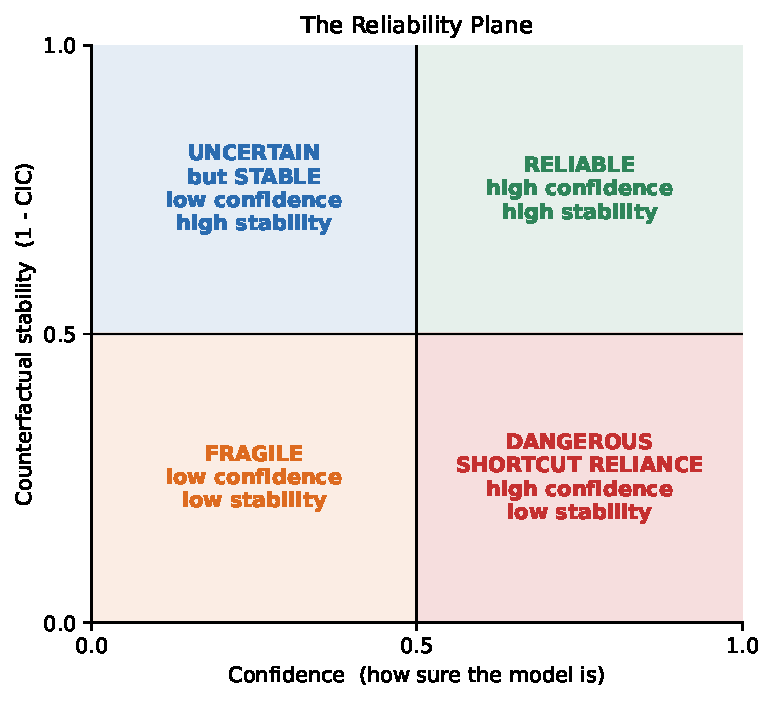
\includegraphics[width=0.62\linewidth]{figures/reliability_plane.pdf}
\caption{The reliability plane. Confidence ($x$) and counterfactual stability ($y$)
are orthogonal axes. The high-confidence / low-stability quadrant (dangerous
shortcut reliance) is invisible to confidence-only monitoring.}
\label{fig:plane}
\end{figure}

% =====================================================================
\section{Experimental Design}\label{sec:design}
% =====================================================================
\paragraph{Model and backend.}
All headline evidence uses real pretrained OpenCLIP zero-shot classification
(\texttt{open\_clip}, \texttt{ViT-B-32}, \texttt{laion2b\_s34b\_b79k}). Every
headline artifact records \texttt{pretrained\_loaded = true} and
\texttt{fake\_backend = false}; results computed under a fallback/fake backend are
structurally blocked from headline eligibility.

\paragraph{Hard multi-decoy benchmark.}
Each image contains a rendered object plus multiple overlaid text regions. In the
\emph{misleading} condition, a harmful word (a competing class name) is overlaid
alongside neutral decoy words; \emph{aligned} overlays carry the true class word;
\emph{no-overlay} images carry the object alone. The benchmark is deliberately hard:
multiple decoys mean a naive ``read the biggest/most-text region'' heuristic is
insufficient.

\paragraph{Non-oracle scoring (leakage control).}
The non-oracle CIC scorer receives only image pixels, CLIP predictions, class
prompts, and a finite set of candidate region proposals. It never sees the true
label, the harmful overlay bounding box, the shortcut type, or per-example
correctness. True labels, oracle neutralization, and bounding boxes are used
\emph{only} to define held-out failure subsets, the oracle upper bound, and
localization metrics --- never inside the scorer.

\paragraph{Repair strategies and baselines.}
CIC region scoring ranks candidate regions by counterfactual instability and
neutralizes the top-$1$/top-$3$ regions (with a \emph{clean-safe} variant that
abstains from edits predicted to harm clean inputs). Controls include matched random
text-region repair (averaged over many random draws), random non-text patch repair,
random augmentation consensus, highest-textness, and largest-text repair. The
\emph{oracle} (known harmful box) repair is reported as an upper bound only.

% =====================================================================
\section{Main Results}\label{sec:results}
% =====================================================================

\subsection{Hard multi-decoy held-out benchmark}
On the current frozen inference path, misleading text reduces natural hard
multi-decoy accuracy from near-perfect clean/aligned performance to the misleading
baseline, and non-oracle CIC improves accuracy substantially over matched random
text-region repair while preserving clean performance (Table~\ref{tab:main},
Figure~\ref{fig:main}).

\begin{table}[t]
\centering
\caption{Hard multi-decoy held-out benchmark, real pretrained OpenCLIP
(\texttt{ViT-B-32}). $n=32$ per condition. Source:
\texttt{results/final\_report/final\_key\_numbers.json}.}
\label{tab:main}
\small
\begin{tabular}{lcc}
\toprule
Condition / method & Accuracy & 95\% CI \\
\midrule
No-overlay & 1.000 & [0.893, 1.000] \\
Aligned overlay & 1.000 & [0.893, 1.000] \\
Misleading (original) & 0.250 & [0.133, 0.421] \\
Oracle harmful-text repair (upper bound) & 1.000 & [0.893, 1.000] \\
\midrule
Matched random text-region repair & 0.331 & $\pm$0.010 (seed) \\
\textbf{CIC top-1 repair} & \textbf{0.750} & [0.579, 0.867] \\
\textbf{CIC top-3 repair} & \textbf{0.750} & [0.579, 0.867] \\
CIC clean-safe repair & 0.750 & [0.579, 0.867] \\
\midrule
CIC top-1 $-$ matched random (gap) & 0.419 & [0.409, 0.430] \\
Clean-safe clean-accuracy drop & 0.010 & --- \\
Top-1 localization IoU $\ge 0.3$ & 0.594 & [0.423, 0.745] \\
Top-1 localization IoU $\ge 0.5$ & 0.063 & --- \\
\bottomrule
\end{tabular}
\end{table}

\begin{figure}[t]
\centering
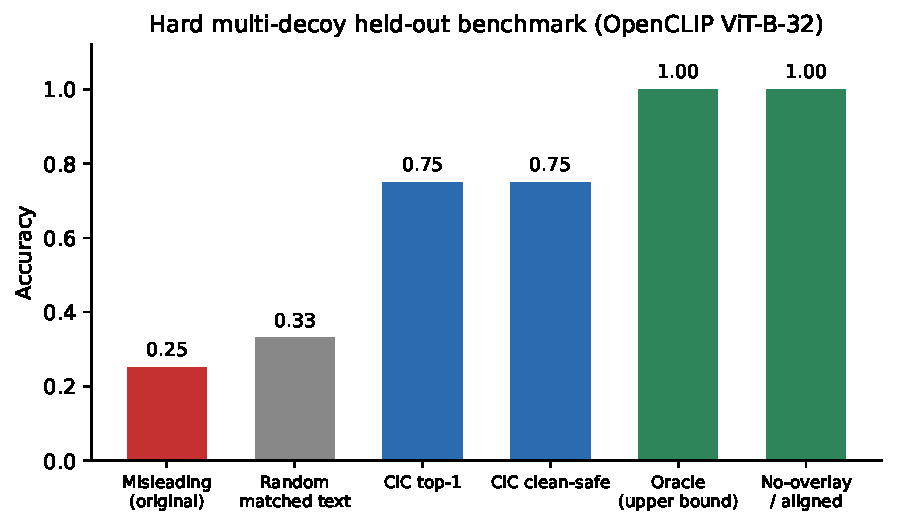
\includegraphics[width=0.78\linewidth]{figures/main_results.pdf}
\caption{Hard multi-decoy benchmark. CIC region scoring ($0.75$) substantially
exceeds matched random text-region repair ($0.33$) and recovers most of the oracle
upper bound ($1.00$), while no-overlay/aligned accuracy is preserved.}
\label{fig:main}
\end{figure}

\paragraph{Selective prediction.}
Adding CIC-guided abstention yields selective accuracy $0.929$ at coverage $0.984$
(2 abstentions, 35 repaired), i.e.\ near-perfect accuracy on covered examples.

\subsection{Full benchmark-resampling audit}
A single fixed benchmark cannot establish stability. We therefore ran a
\emph{full benchmark-resampling audit}: three independently resampled held-out
benchmark instances, each with a new object sequence, harmful class, decoy words,
placements, image IDs, and \emph{distinct image-set and metadata hashes}, evaluated
under frozen generation and repair policies. This addresses an earlier limitation in
which only a fixed-benchmark determinism check was available.

\begin{table}[t]
\centering
\caption{Full benchmark-resampling audit ($3$ resampled instances, distinct image/
metadata hashes). Source:
\texttt{results/hard\_multidecoy\_clip\_repair/full\_benchmark\_resampling\_*}.}
\label{tab:resample}
\small
\begin{tabular}{lccc}
\toprule
Quantity & Mean & Min & Max \\
\midrule
Original misleading accuracy & 0.260 & 0.250 & 0.281 \\
CIC top-1 repair & 0.750 & 0.719 & 0.813 \\
Matched random text repair & 0.289 & 0.268 & 0.329 \\
CIC $-$ random gap & 0.461 & 0.390 & 0.545 \\
Clean-safe clean drop & 0.014 & --- & --- \\
\bottomrule
\end{tabular}
\end{table}

All three seeds were benchmark-resampled with unique hashes, all had original
accuracy $\le 0.40$, all had CIC beating random by $\ge 0.15$, and
\texttt{full\_benchmark\_resampling\_stability\_supported = true}. The effect is
stable across resampled benchmark instances, not an artifact of one fixed draw.

\subsection{Scale and multi-model replication audit}
As supporting evidence (this does \emph{not} replace the frozen primary headline,
which remains \texttt{ViT-B-32}~/~\texttt{laion2b\_s34b\_b79k} at $n=32$ per
condition), we ran a scale-and-multi-model replication audit at
$n_{\text{per condition}}=128$. Four real pretrained OpenCLIP backbone/checkpoint
pairs were attempted; all four loaded (none skipped, no fake backend), and all
four were \texttt{repair\_eligible}. All four models were evaluated on the
\emph{same} larger resampled benchmark instance (one shared benchmark hash) for a
fair cross-model comparison; that benchmark hash differs from the $n=32$ headline
benchmark, so these values are a separate larger-$n$ replication rather than a
cell-for-cell restatement of the headline. The test suite passes ($186$ tests).

\begin{table}[t]
\centering
\caption{Scale and multi-model replication audit ($n_{\text{per condition}}=128$;
four pretrained OpenCLIP backbone/checkpoint pairs on one shared resampled
benchmark instance). Source:
\texttt{results/hard\_multidecoy\_scale\_model\_audit/scale\_model\_metrics.csv}.}
\label{tab:scalemodel}
\small
\begin{tabular}{llccccc}
\toprule
Model & Pretrained & Orig.\ misl. & CIC top-1 & Matched rand. & Gap & Clean drop \\
\midrule
ViT-B-32 & laion2b\_s34b\_b79k & 0.289 & 0.742 & 0.305 & 0.437 & 0.036 \\
ViT-B-32 & openai & 0.062 & 0.688 & 0.111 & 0.576 & 0.003 \\
ViT-B-16 & laion2b\_s34b\_b88k & 0.078 & 0.938 & 0.159 & 0.778 & 0.000 \\
RN50 & openai & 0.000 & 0.758 & 0.072 & 0.686 & 0.000 \\
\bottomrule
\end{tabular}
\end{table}

The main text-overlay result is stable at larger $n$, and the text-overlay CIC
effect replicates across multiple pretrained OpenCLIP backbones/checkpoints. This
audit does \emph{not} imply open-world shortcut discovery, general robustness,
cross-shortcut generalization, or exact localization: the method still searches a
finite candidate class of text-region proposals on a controlled synthetic
text-overlay benchmark. The frozen primary headline (Table~\ref{tab:main}) is
unchanged.

\subsection{Second shortcut family: non-text semantic-decoy icon}
As positive supporting evidence---not a replacement for the text-overlay
headline---we re-ran the same finite-candidate CIC region method, from scratch
(not a frozen transfer), on an independent non-text shortcut family. Each stimulus
contains a central colored \emph{causal} icon (the true label) and a larger,
spatially separated, competing-class \emph{decoy} icon in a corner, with no written
words anywhere. The decoy's oracle box is used only for the oracle upper bound and a
diagnostic IoU; the non-oracle scorer sees only pixels, candidate boxes, and model
probabilities. On real pretrained OpenCLIP \texttt{ViT-B-32}~/~\texttt{laion2b\_s34b\_b79k}
(fake backend blocked), the decoy drives misleading-regime accuracy to $0.297$
while the central icon alone is perfectly recognized (clean $1.000$) and oracle
removal of the decoy fully restores it ($1.000$). The $n=64$ pilot passed all $8$
strict gates, and the $n=128$ scale run also passed all $8$ gates (no failed
gates), so the result is stable across scale.

\begin{table}[t]
\centering
\caption{Second shortcut family (non-text semantic-decoy icon), $n_{\text{per
condition}}=128$, real pretrained OpenCLIP \texttt{ViT-B-32}~/~\texttt{laion2b\_s34b\_b79k}.
Source: \texttt{results/semantic\_decoy\_scale\_n128/semantic\_decoy\_pilot\_gates.json}.}
\label{tab:semdecoy}
\small
\begin{tabular}{lc}
\toprule
Quantity (misleading regime unless noted) & Value \\
\midrule
Clean / no-shortcut accuracy & 1.000 \\
Misleading original accuracy & 0.297 \\
Oracle decoy neutralization (upper bound) & 1.000 \\
\textbf{CIC top-1 repair} & \textbf{0.711} \\
CIC top-3 repair & 0.359 \\
CIC clean-safe repair & 0.766 \\
Matched random candidate repair & 0.258 \\
CIC $-$ random gap & 0.453 \\
Clean-safe clean drop & 0.008 \\
\bottomrule
\end{tabular}
\end{table}

CIC thus succeeds on a second controlled finite-candidate shortcut family beyond
text overlays under controlled oracle-intervention conditions, with the same
gating discipline. This does \emph{not} imply open-world shortcut discovery,
general robustness, cross-shortcut transfer, universal shortcut repair, or exact
localization; it is a single-model, single-family controlled result. An earlier
flat visual-decoy pilot was not failure-rich enough (its single low-salience
competing shape only drove misleading accuracy to ${\sim}0.58$, exceeding the
$\le 0.40$ failure gate) and is retained as boundary evidence; the semantic-decoy
icon benchmark was the final pre-specified second-family attempt and passed all
gates.

\subsection{Failure-conditioned benchmark}
To probe repair precisely where the model fails, we built a failure-conditioned
subset. From $76$ generated candidates, $50$ verified failures were admitted
(inclusion rate $0.658$) under the predicate: pretrained CLIP classifies the
\emph{no-overlay} and \emph{aligned} images correctly, classifies the
\emph{misleading} image incorrectly with confidence $\ge 0.5$, \emph{and} oracle
harmful-text neutralization restores the correct prediction. By construction the
original failure-subset accuracy is $0$ --- this is \emph{not} a natural accuracy and
does not establish general robustness or discovery. We restate this caveat wherever
the number appears.

\begin{table}[t]
\centering
\caption{Failure-conditioned repair on $50$ verified shortcut failures (original
accuracy $=0$ by construction). Source:
\texttt{results/hard\_multidecoy\_failure\_conditioned/}.}
\label{tab:failcond}
\small
\begin{tabular}{lcc}
\toprule
Method & Repaired accuracy & 95\% CI \\
\midrule
Original (by construction) & 0.000 & [0.000, 0.071] \\
Oracle harmful-text repair (upper bound) & 1.000 & [0.929, 1.000] \\
\textbf{CIC top-1 repair} & \textbf{0.960} & [0.865, 0.989] \\
\textbf{CIC top-3 repair} & \textbf{0.980} & [0.893, 0.996] \\
CIC clean-safe repair & 0.940 & [0.838, 0.979] \\
Highest-textness repair & 0.820 & [0.692, 0.902] \\
Largest-text repair & 0.260 & [0.159, 0.396] \\
Matched random text-region repair & 0.112 & $\pm$0.015 \\
Random augmentation consensus & 0.020 & [0.004, 0.105] \\
Random non-text patch repair & 0.002 & [0.001, 0.007] \\
\bottomrule
\end{tabular}
\end{table}

CIC repairs $96$--$98\%$ of verified failures versus $\approx 11.2\% \pm 1.5\%$ for
matched random text repair (gap $0.868$, non-overlapping CIs); clean and aligned
preservation after clean-safe repair are both $1.000$. Localization is $0.82$ (top-1)
and $0.90$ (top-3) at coarse IoU $\ge 0.3$ but only $0.04$ at IoU $\ge 0.5$. The
repair-vs-localization crosstab shows repair is near-certain when coarse
localization succeeds (IoU $\ge 0.3$: CIC top-1 $=1.0$) and \emph{still often
succeeds} when it does not (IoU $<0.3$, $n=9$: CIC top-1 $=0.78$). We therefore claim
\emph{coarse causal-region intervention}, not exact box localization.

\begin{figure}[t]
\centering
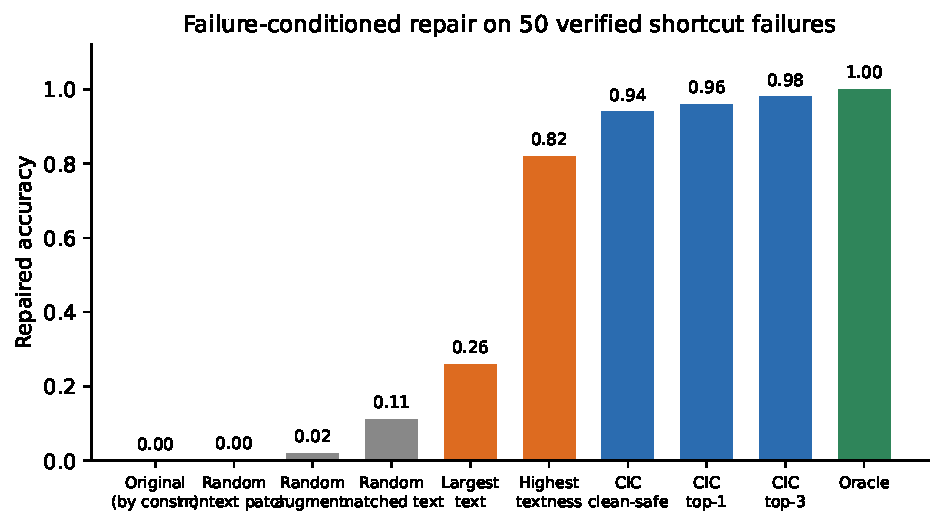
\includegraphics[width=0.82\linewidth]{figures/failure_conditioned.pdf}
\caption{Failure-conditioned repair. CIC variants ($0.94$--$0.98$) approach the
oracle upper bound ($1.00$); all random and generic controls remain low, with
matched random text repair at $0.112$.}
\label{fig:failcond}
\end{figure}

% =====================================================================
\section{Theory and Mechanism}\label{sec:theory}
% =====================================================================
We state a conditional, finite-candidate recovery theory and report whether its
assumptions hold for OpenCLIP. The theory explains \emph{when} neutralizing a
shortcut region restores the causal prediction; it does not prove discovery, exact
localization, or robustness.

\subsection{Additive-channel assumption}
We assume the per-class logit decomposes into a causal channel, a shortcut channel,
and a small interaction residual:
\begin{equation}\label{eq:additive}
\ell_y\big(g(C,S,N)\big) = \phi_y(C,N) + \psi_y(S) + \xi_y(C,S,N).
\end{equation}
For zero-shot CLIP, logits are inner products $\ell_y(X)=\langle u(X), v_y\rangle$,
so \eqref{eq:additive} is additive in the embedding exactly when the embedding is
additive: the shortcut channel $\psi_y(S)=\langle \delta_S, v_y\rangle$ has a
well-defined, approximately \emph{input-independent} direction $\delta_S$ iff
$u(\text{object}+\text{shortcut}) - u(\text{object}) \approx \delta_S$ independent of
the object. This reduces the assumption to a measurable claim about embedding
geometry.

\subsection{Exact and approximate recovery}
\begin{theorem}[Exact neutralization]
If \eqref{eq:additive} holds with $\xi_y\equiv 0$ and the neutral value $s_0$ makes
the shortcut channel class-independent ($\psi_y(s_0)=c$ for all $y$), then
$\argmax_y[\phi_y(C,N)+\psi_y(s_0)] = \argmax_y \phi_y(C,N)$. Neutralization recovers
the causal argmax.
\end{theorem}
A class-independent offset cannot change which class wins. Allowing residual error,
let the causal margin be $m(X)=\phi_{y^*}(C,N)-\max_{y\ne y^*}\phi_y(C,N)$ and bound
the causal-channel damage, residual shortcut, and interaction by
$\epsilon_C,\epsilon_S,\epsilon_\xi$.
\begin{theorem}[Approximate recovery]
If $m(X) > 2(\epsilon_C+\epsilon_S+\epsilon_\xi)$, then the post-neutralization
argmax equals the causal argmax $y^*$.
\end{theorem}
Each error term moves a score by at most its bound; the worst-case winner/runner-up
swing is twice the summed bounds.

\subsection{Class-balanced sweep corollary}
Averaging logits over a class-balanced sweep $B$ of shortcut values,
$\bar f_y(X)=\frac{1}{|B|}\sum_{s\in B}\ell_y(g(C,s,N))$, cancels the shortcut
contribution up to a class-independent offset whenever the average shortcut channel
$\frac{1}{|B|}\sum_{s\in B}\psi_y(s)$ is class-independent --- the basis for
consensus/sweep repair.

\subsection{Object-entanglement: the global form fails for CLIP}
The embedding-additivity validation tests the \emph{strong, global} form of
\eqref{eq:additive} on real OpenCLIP. The result is a negative-but-informative
structural finding (Table~\ref{tab:theory}, Figure~\ref{fig:entangle}):
\begin{quote}
\itshape OpenCLIP's typographic shortcut effect is not a single global additive bias
direction. The shift induced by overlay text is \textbf{object-entangled}: it
contains a real shortcut component, but its direction varies substantially with the
underlying object.
\end{quote}
Concretely, same-shortcut deltas cluster above the shuffled-label baseline
(within-shortcut cosine $0.765$ vs.\ shuffled $0.634$), confirming a real shortcut
component, and the logit decomposition is exactly additive in embedding space
(consistency MAE $\approx 6\times10^{-15}$). \emph{But} the per-image delta clusters
\emph{more} tightly by object class than by shortcut value (within-object cosine
$0.855 > 0.765$), so $\delta_S$ is not input-independent, and the neutralization
damage is not small relative to the multi-decoy shortcut effect (ratio $0.92$).
Hence \texttt{embedding\_additivity\_supported\_for\_text = false}: the global
additivity theorem is \textbf{not} claimed to apply to CLIP. This explains why
generic global debiasing is unlikely to suffice, while targeted per-input region
scoring still repairs failures.

\subsection{Per-input residual-to-clean class-balance: the weaker premise the theorem needs}
Global additivity is stronger than recovery requires, and the relevant baseline is
the \emph{clean} prediction, not the misleading input. Let $x_{\mathrm{clean}}$ be
the no-overlay/clean image with the same causal content, and let $T(x)$ be the
neutralized/repaired version of the misleading image. Define the per-class
\textbf{residual-to-clean}
\begin{equation}
\rho_y(x) = \ell_y\big(T(x)\big) - \ell_y\big(x_{\mathrm{clean}}\big),
\qquad
\bar\rho(x) = \frac{1}{|\mathcal{Y}|}\sum_{y\in\mathcal{Y}}\rho_y(x).
\end{equation}
The \textbf{per-input residual-to-clean class-balance condition} is
\begin{equation}
\max_{y\in\mathcal{Y}} \big|\rho_y(x)-\bar\rho(x)\big| \le \epsilon_B,
\end{equation}
which allows the shortcut effect to vary across inputs as long as the repaired
logits differ from the clean logits by an approximately class-independent residual
\emph{within} each input. We define the residual relative to the clean/causal
logits, not relative to the misleading input logits: a shift that is class-balanced
relative to the misleading logits would preserve the misleading argmax, whereas
recovery requires returning to the clean causal argmax.

\begin{corollary}[Per-input residual-to-clean recovery]
If the repaired logits differ from the clean logits by an approximately
class-independent residual ($\max_y|\rho_y(x)-\bar\rho(x)|\le\epsilon_B$) and the
clean causal margin satisfies $m_{\mathrm{clean}}(x)>2\epsilon_B$, then
\begin{equation}
\argmax_y \ell_y\big(T(x)\big) = \argmax_y \ell_y\big(x_{\mathrm{clean}}\big).
\end{equation}
\end{corollary}
\begin{proof}[Proof sketch]
Write $\ell_y(T(x))=\ell_y(x_{\mathrm{clean}})+\bar\rho(x)+r_y(x)$ with
$|r_y(x)|\le\epsilon_B$. The common offset $\bar\rho(x)$ shifts all classes equally
and cannot change the argmax; the residual can shrink the clean winner's margin by at
most $2\epsilon_B$. Hence if $m_{\mathrm{clean}}(x)>2\epsilon_B$, the clean winner
remains the repaired winner.
\end{proof}

The earlier global additivity test asked whether overlay-induced embedding shifts
were input-independent across images. The residual-to-clean test is weaker and more
directly tied to recovery: it asks whether a particular neutralization leaves the
repaired logits close to the clean logits up to an approximately class-independent
offset. This is the quantity reported in Table~\ref{tab:theory}, measured in
residual-to-clean logit units.

This weaker premise \emph{is} supported on OpenCLIP text overlays
(\texttt{per\_input\_class\_balance\_supported\_for\_text = true},
\texttt{clip\_theory\_support\_status = ``CLIP-supported via per-input
class-balance''}). With $\epsilon_B=3.0$ logits, oracle and CIC neutralization are
substantially more class-balanced (lower residual-to-clean) than matched random
text-region neutralization, and the margin condition tracks repair success: when
satisfied, repair succeeds $100\%$ of the time across all conditions
(Table~\ref{tab:theory}, Figure~\ref{fig:classbal}). The mechanism is validated most
tightly for oracle neutralization and approximately for CIC. Because CIC's median
residual-to-clean ($\approx 3.7$ top-1, $\approx 3.5$ top-3) exceeds
$\epsilon_B=3.0$, the theorem does not fully explain every CIC success: CIC
neutralization is more class-balanced than matched random repair and aligns with the
recovery condition directionally, but the worst-case margin condition is
conservative, and many successful CIC repairs occur even when the sufficient
condition is not formally satisfied.

\begin{table}[t]
\centering
\caption{Theory validation. Top: global embedding additivity (not supported).
Bottom: per-input class-balance (supported for text). Sources:
\texttt{results/embedding\_additivity/} and \texttt{results/per\_input\_class\_balance/}.}
\label{tab:theory}
\small
\begin{tabular}{lcccc}
\toprule
\multicolumn{5}{l}{\textit{Global embedding additivity} (\texttt{supported\_for\_text = false})}\\
\midrule
\multicolumn{3}{l}{within-shortcut cosine} & 0.765 & \\
\multicolumn{3}{l}{shuffled-label baseline cosine} & 0.634 & \\
\multicolumn{3}{l}{within-object cosine ($>$ within-shortcut)} & 0.855 & \\
\multicolumn{3}{l}{neutralization damage / shortcut-effect ratio} & 0.917 & \\
\multicolumn{3}{l}{logit-channel consistency MAE} & $6{\times}10^{-15}$ & \\
\midrule
\multicolumn{5}{l}{\textit{Per-input class-balance} (\texttt{supported\_for\_text = true}, $\epsilon_B=3.0$)}\\
\midrule
Condition & Median residual & Repair acc. & Margin-cond.\ rate & \\
\midrule
Oracle & 2.464 & 1.000 & 0.719 & \\
CIC top-1 & 3.704 & 0.781 & 0.344 & \\
CIC top-3 (consensus) & 3.506 & 0.781 & 0.344 & \\
Matched random text & 5.220 & 0.406 & 0.125 & \\
\bottomrule
\end{tabular}
\end{table}

\begin{figure}[t]
\centering
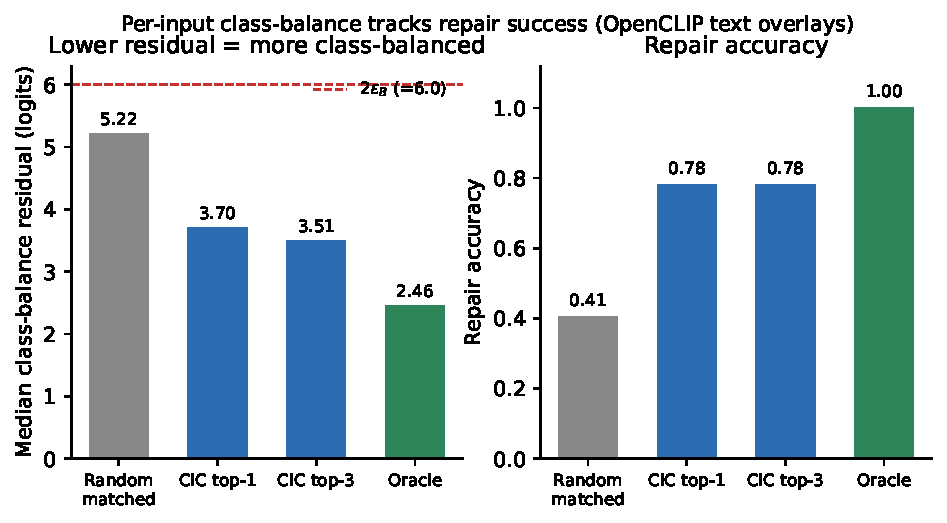
\includegraphics[width=0.95\linewidth]{figures/class_balance.pdf}
\caption{Per-input class-balance. Oracle and CIC neutralization produce lower (more
class-balanced) residuals than matched random neutralization, and correspondingly
higher repair accuracy. The dashed line marks the recovery threshold $2\epsilon_B$.}
\label{fig:classbal}
\end{figure}

\begin{figure}[t]
\centering
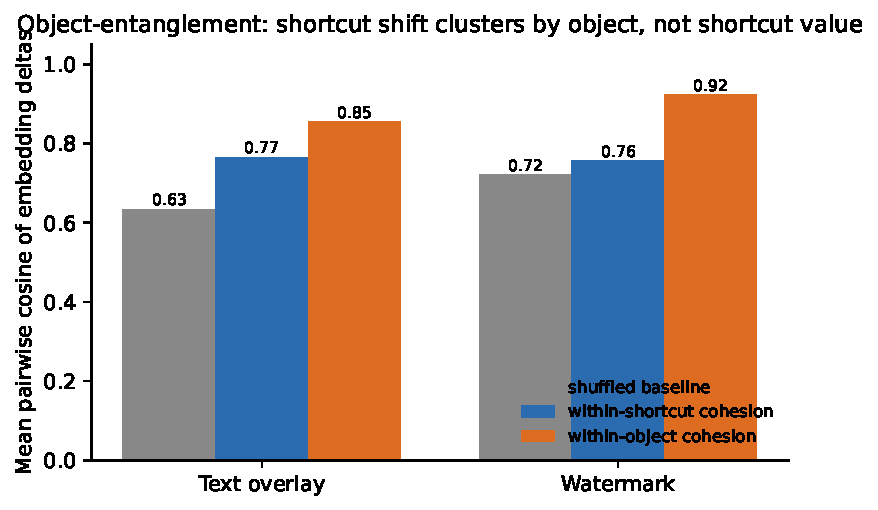
\includegraphics[width=0.72\linewidth]{figures/object_entanglement.pdf}
\caption{Object-entanglement. For both shortcut families the per-image embedding
shift clusters more tightly by object class than by shortcut value, so the shortcut
direction is not a single global bias direction. For the watermark the
within-shortcut cohesion barely exceeds the shuffled baseline (weak/flat channel).}
\label{fig:entangle}
\end{figure}

\paragraph{Repair advantage over matched random.}
Heuristically, the expected gap between CIC and a matched random control,
$\mathbb{E}[\mathrm{CIC}]-\mathbb{E}[\mathrm{random}]\approx
\big(q-\tfrac{r}{m}\big)(p_u-p_d)$, increases with the probability $q$ that CIC ranks
the true shortcut region highly relative to the fraction $r/m$ of useful regions a
random draw hits, scaled by the difference between up-repair and down-repair
probabilities. The measured gaps ($0.42$ main, $0.46$ resampled, $0.87$
failure-conditioned) are consistent with CIC's region ranking being substantially
better than chance.

\paragraph{Interpretation.}
The theorem's variable is \emph{low causal-channel damage}, not exact IoU: a coarse
region that covers the shortcut while leaving the object intact yields small
$\epsilon_C$. This is why repair succeeds at coarse IoU $\ge 0.3$ while exact IoU
$\ge 0.5$ stays weak. The account is conditional and finite-candidate only.

% =====================================================================
\section{Negative Results and Boundary Conditions}\label{sec:negative}
% =====================================================================
We retain negative results rather than hide them.

\paragraph{Cross-shortcut transfer fails (watermarks).}
We froze the text-overlay-selected CIC policy and applied it, \emph{with no
retuning}, to a non-text colored-symbol watermark shortcut on real OpenCLIP. In the
natural benchmark, CLIP barely reads the watermark (original misleading accuracy
$0.75$, i.e.\ the shortcut is weak), and in the failure-conditioned mode only $4$ of
$384$ candidates ($1.0\%$) met the failure predicate. The frozen CIC repair reached
only $0.50$ on that tiny subset; \texttt{cross\_shortcut\_headline\_eligible =
false} (failure reasons: too few failures and natural accuracy not low enough;
frozen CIC top-1/3 $<0.70$; clean preservation not high). \textbf{We claim no
cross-shortcut generalization.} The main claim remains text-region finite-candidate
repair. The embedding-additivity validation explains this: the watermark shortcut
channel is weak/flat (within-object cosine $0.923 \gg$ within-shortcut $0.757$,
\texttt{watermark\_shortcut\_channel\_weak = true}), so there is little shortcut
contribution to neutralize --- a transfer failure \emph{consistent with} the theory
rather than a refutation.

\begin{table}[t]
\centering
\caption{Negative and boundary results. Sources:
\texttt{results/cross\_shortcut\_generalization/} and
\texttt{results/embedding\_additivity/}.}
\label{tab:negative}
\small
\begin{tabular}{lcc}
\toprule
Result & Value & Status \\
\midrule
Cross-shortcut natural misleading accuracy & 0.750 & shortcut weak \\
Cross-shortcut failure inclusion rate & 0.010 (4/384) & too few failures \\
Cross-shortcut frozen CIC top-1 (failure subset) & 0.500 & below threshold \\
Cross-shortcut headline eligible & false & \textbf{no transfer} \\
\midrule
Global additivity supported (text) & false & object-entangled \\
Global additivity supported (watermark) & false & weak channel \\
Exact localization IoU $\ge 0.5$ (main) & 0.063 & coarse only \\
\bottomrule
\end{tabular}
\end{table}

\paragraph{No exact localization; no general robustness.}
Localization is strong at coarse IoU $\ge 0.3$ and weak at IoU $\ge 0.5$ across all
settings, so we claim coarse causal-region localization only. The benchmark is
controlled and generated; we make no broad real-world robustness claim.

% =====================================================================
\section{Codebase and Reproducibility Audit}\label{sec:repro}
% =====================================================================
\paragraph{Repository structure.}
The codebase separates concerns: experiment runners
(\texttt{causal\_reliability/experiments/}), discovery and region scoring
(\texttt{causal\_reliability/discovery/}), repair and abstention
(\texttt{causal\_reliability/repair/}), validation
(\texttt{causal\_reliability/validation/}), an audit API
(\texttt{causal\_reliability/api/}, \texttt{causal\_reliability/audit/}), and real
models (\texttt{causal\_reliability/real\_models/}). Experiments are config-driven
(\texttt{configs/*.yaml}), and every run writes structured artifacts (CSV/JSON/MD
plus plots) under \texttt{results/}. The final report and machine-readable key
numbers are regenerated into \texttt{results/final\_report/}.

\paragraph{Reproducibility controls.}
The hard multi-decoy audit distinguishes a fixed-benchmark determinism check from
true benchmark resampling. The full benchmark-resampling audit draws independent
held-out instances and records distinct \texttt{image\_set\_hash} and
\texttt{metadata\_hash} per seed; identical hashes would invalidate a stability
claim. Caching/resume is artifact-based, and timing profiles are recorded.

\paragraph{Leakage prevention.}
The non-oracle scorer is structurally denied the true label, harmful bbox, shortcut
type, and correctness; these are used only to define failure subsets, oracle bounds,
and localization metrics. A fallback/fake backend is blocked from headline
eligibility, and headline flags (\texttt{headline\_eligible}) are gated on pretrained
loading, leakage checks, low original accuracy, beating matched random, and clean
preservation.

\paragraph{Artifact-derived reporting and tests.}
The paper's numbers are taken from regenerated artifacts (chiefly
\texttt{final\_key\_numbers.json}), not from earlier exploratory runs. The test suite
passes \textbf{174/174} (\texttt{python3 -m pytest}), and includes tests for
no-oracle-leakage, cross-shortcut generalization gating, embedding-additivity/theory
gating, per-input class-balance, and final-report caveats. The repository's
$24/24$ negative controls pass.

\paragraph{Stale-number fix.}
An earlier exploratory headline (a $0.219 \to 0.875$ / $28.8\%$ figure) was produced
under a previous prediction path and is \emph{not} used here. The
\texttt{FINAL\_ARTIFACT\_INDEX.md} ``Final Headline Result'' block now reports the
authoritative current numbers and confines the earlier figure to a clearly marked
``Historical stale exploratory result --- not current headline'' subsection. The
authoritative current artifacts (\texttt{final\_key\_numbers.json}) report
$0.250 \to 0.750$ with matched random $0.331$, and this paper uses those. See
Appendix~\ref{app:stale} for the discrepancy note.

\paragraph{Human label-preservation validation.}
Three annotators evaluated $100$ original/repaired image pairs ($300$ total
annotations). Majority vote found that the object label was preserved in $96$ of $100$
pairs and that the repaired image remained recognizable in $97$ of $100$ pairs.
Inter-annotator agreement was high: Fleiss' $\kappa$ was $0.973$ for before-label
judgments, $0.974$ for after-label judgments, $0.920$ for whether the label changed,
and $1.000$ for after-image recognizability (percent agreement $0.980$, $0.980$,
$0.993$, and $1.000$ respectively). The four preservation failures were retained and
flagged rather than removed
(\texttt{results/human\_label\_preservation/human\_validation\_flags.csv}): one apparent
shape change (square$\rightarrow$circle, still recognizable), one blurry/unrecognizable
repair, one corrupted/glitched repair, and one blank/missing-shape repair. The analysis
pipeline (\texttt{validation/human\_label\_preservation/analyze\_annotations.py})
computes these majority-vote rates, percent agreement, and Fleiss' kappa for the
before-label, after-label, label-change, and recognizability fields directly from the
raw per-annotator responses. Before/after label accuracy against the true label is
reported only when pair-level true labels (\texttt{metadata\_hidden.csv}) are present,
and is otherwise left as n/a; no true labels were fabricated.

\paragraph{WILDS Waterbirds metadata-only diagnostic.}
WILDS Waterbirds was also parsed as a real spurious-background diagnostic. A
metadata-only OpenCLIP evaluation showed the expected background sensitivity: overall
accuracy was $56.0\%$, with land-background accuracy $73.1\%$ versus water-background
accuracy $35.9\%$, and landbird accuracy dropping from $74.4\%$ on land backgrounds to
$21.6\%$ on water backgrounds. However, WILDS Waterbirds does not ship
oracle-repairable bird/background masks or bounding boxes, so CIC repair and
failure-conditioned oracle repair were not run. This diagnostic motivates a future
regenerated CUB+Places Waterbirds-style benchmark with known masks, but it is
\emph{not} a positive CIC repair result and is not part of the main results.

\paragraph{Honest limitations of the codebase.}
The full benchmark-resampling audit used a reduced number of random-baseline repeats
per seed to bound runtime (each seed $\approx 9$ minutes), so per-seed random-baseline
CIs are wider than the main run's $100$-seed estimate. The failure-conditioned and
cross-shortcut evaluations are small-$n$ by construction. The human label-preservation
study (three annotators, $100$ pairs) was performed on text-overlay repair pairs;
broader validation across other shortcut families and real-world datasets remains
future work.

% =====================================================================
\section{Limitations}\label{sec:limits}
% =====================================================================
\begin{itemize}[leftmargin=1.4em,itemsep=2pt]
\item \textbf{Finite candidate class only.} CIC tests the intervention family it is
given; it is \textbf{not} open-world shortcut discovery.
\item \textbf{No exact localization.} Coarse causal-region localization (IoU
$\ge 0.3$) only; IoU $\ge 0.5$ is weak.
\item \textbf{No general robustness.} Results are on controlled, generated
benchmarks with one pretrained CLIP model.
\item \textbf{No cross-shortcut transfer.} The text-region policy did not transfer to
the watermark shortcut.
\item \textbf{Failure-conditioned conditioning.} The $96$--$98\%$ repair is on a
subset where CLIP already fails (original accuracy $0$ by construction); it is not a
natural accuracy.
\item \textbf{Theory caveat.} Global input-independent additivity failed; the theory
is supported only via the weaker per-input class-balance premise.
\item \textbf{Human validation.} Human label-preservation validation was performed on
$100$ text-overlay repair pairs with three annotators (majority-vote object label
preserved in $96/100$, repaired image recognizable in $97/100$; Fleiss' $\kappa$ up to
$1.000$); broader validation across other shortcut families and real-world datasets
remains future work.
\item \textbf{Real spurious-background diagnostic only.} WILDS Waterbirds was parsed as
a real spurious-background diagnostic and OpenCLIP showed the expected background
sensitivity (overall $56.0\%$; land $73.1\%$ vs.\ water $35.9\%$; landbird $74.4\%$ on
land vs.\ $21.6\%$ on water). However, WILDS Waterbirds does not ship oracle-repairable
masks/bboxes, so CIC repair was not run on it. A regenerated CUB+Places
Waterbirds-style pilot with known masks was implemented but remained gated on missing
external assets in the current run. Therefore Waterbirds is motivation/future work, not
a positive CIC repair result.
\end{itemize}

% =====================================================================
\section{Conclusion}\label{sec:conclusion}
% =====================================================================
Confidence measures how sure a model is; it cannot distinguish uncertainty from
shortcut dependence. Counterfactual stability provides a second axis. On real
pretrained OpenCLIP, finite-candidate text-region CIC repair beats matched controls
across the hard held-out benchmark ($0.25\to0.75$ vs.\ $0.33$ random), a full
benchmark-resampling audit (gap $0.39$--$0.54$), and a failure-conditioned evaluation
($96$--$98\%$ vs.\ $11.2\%$). The mechanism is explained not by a global additive
shortcut direction --- which fails because the typographic effect is
object-entangled --- but by the weaker per-input class-balance condition the recovery
theorem actually requires, which is supported. The boundary is equally clear: the
frozen policy does not transfer to a weak-channel watermark shortcut. The result is a
finite-candidate audit-and-repair framework, not general shortcut discovery.

% =====================================================================
\appendix
\section{Appendix: Stale-Number Discrepancy Note}\label{app:stale}
% =====================================================================
An earlier exploratory headline reported $0.219\to0.875$ with matched random $0.288$
under a prior prediction path. That value is not used in this paper. The
authoritative current artifact,
\texttt{results/final\_report/final\_key\_numbers.json}, reports original misleading
accuracy $0.250$, CIC top-1 repair $0.750$, and matched random repair $0.331$
(\texttt{hard\_multidecoy\_headline\_primary\_metric = "misleading accuracy 0.250 to
0.750"}). The artifact index (\texttt{FINAL\_ARTIFACT\_INDEX.md}) has been updated to
mark the earlier value as stale historical context rather than as the final result,
so the repository is now internally consistent on this number.

\section{Appendix: Artifact-to-Number Map}\label{app:map}
\small
\begin{tabular}{p{0.40\linewidth}p{0.54\linewidth}}
\toprule
Number(s) used & Source artifact \\
\midrule
Hard multi-decoy main table & \texttt{results/final\_report/final\_key\_numbers.json} \\
Full resampling audit (3 seeds) & \texttt{.../hard\_multidecoy\_clip\_repair/full\_benchmark\_resampling\_aggregate.csv} and \texttt{\_audit.csv} \\
Scale + multi-model audit ($n{=}128$, 4 models) & \texttt{.../hard\_multidecoy\_scale\_model\_audit/scale\_model\_metrics.csv}, \texttt{scale\_model\_key\_numbers.json}, \texttt{scale\_model\_summary.md}, \texttt{scale\_model\_plot.png}, \texttt{model\_availability.csv} \\
Second shortcut family (semantic-decoy icon, $n{=}64$ \& $n{=}128$) & \texttt{.../semantic\_decoy\_pilot/semantic\_decoy\_pilot\_gates.json}, \texttt{.../semantic\_decoy\_scale\_n128/semantic\_decoy\_pilot\_gates.json}; \texttt{final\_key\_numbers.json} (\texttt{semantic\_decoy\_*}) \\
Failure-conditioned table & \texttt{.../hard\_multidecoy\_failure\_conditioned/failure\_conditioned\_metrics.csv}, \texttt{\_key\_numbers.json} \\
Cross-shortcut negative result & \texttt{.../cross\_shortcut\_generalization/cross\_shortcut\_summary.md}, \texttt{final\_key\_numbers.json} \\
Global additivity & \texttt{.../embedding\_additivity/embedding\_additivity\_key\_numbers.json} \\
Per-input class-balance & \texttt{.../per\_input\_class\_balance/per\_input\_class\_balance\_key\_numbers.json} \\
Confident-wrong / confidence-solvable AUROCs & \texttt{results/final\_report/final\_key\_numbers.json} \\
Dangerous quadrant count / rate & \texttt{final\_key\_numbers.json} (\texttt{dangerous\_quadrant\_*}) \\
Tests / negative controls & \texttt{python3 -m pytest}; \texttt{final\_key\_numbers.json} (\texttt{negative\_controls\_*}) \\
\bottomrule
\end{tabular}

\section{Appendix: Reproducibility Checklist}\label{app:checklist}
\small
\begin{tabular}{p{0.74\linewidth}c}
\toprule
Item & Status \\
\midrule
Real pretrained OpenCLIP loaded (no fake backend for headline) & yes \\
Non-oracle scorer excludes label/bbox/type/correctness & yes \\
Headline gated on \texttt{headline\_eligible} & yes \\
Full benchmark resampling with distinct image/metadata hashes & yes (3 seeds) \\
Scale + multi-model replication audit (supporting, $n{=}128$) & yes (4/4 loaded, all repair-eligible) \\
\quad shared resampled benchmark instance across models; hash $\ne$ $n{=}32$ headline & yes \\
Fixed-benchmark determinism check separated from resampling & yes \\
Global-additivity theory claim gated on validation metric & yes (false) \\
Per-input class-balance gate & yes (true for text) \\
Cross-shortcut transfer reported honestly when failing & yes (not eligible) \\
Second shortcut family (semantic-decoy icon; supporting, not headline) & yes ($n{=}64$ \& $n{=}128$ both 8/8 gates) \\
\quad earlier flat visual-decoy pilot retained as boundary evidence & yes (1 gate fails) \\
Test suite & 186/186 pass \\
Negative controls & 24/24 pass \\
Human label-preservation study (3 annotators, 100 pairs) & yes \\
\quad majority-vote label preserved / recognizable & 96/100, 97/100 \\
\quad Fleiss' $\kappa$ (before/after/change/recognizable) & 0.973 / 0.974 / 0.920 / 1.000 \\
WILDS Waterbirds (metadata-only diagnostic; no CIC repair) & diagnostic \\
\bottomrule
\end{tabular}

\bibliographystyle{plain}
\bibliography{references}

\end{document}
